\documentclass[journal,12pt,twocolumn]{IEEEtran}
\usepackage{setspace}
\usepackage{gensymb}
\usepackage{xcolor}
\usepackage{caption}
%\usepackage{subcaption}
%\doublespacing
\singlespacing
%\usepackage{graphicx}
%\usepackage{amssymb}
%\usepackage{relsize}
\usepackage[cmex10]{amsmath}
\usepackage{mathtools}
%\usepackage{amsthm}
%\interdisplaylinepenalty=2500
%\savesymbol{iint}
%\usepackage{txfonts}
%\restoresymbol{TXF}{iint}
%\usepackage{wasysym}
\usepackage{hyperref}
\usepackage{amsthm}
\usepackage{mathrsfs}
\usepackage{txfonts}
\usepackage{stfloats}
\usepackage{cite}
\usepackage{cases}
\usepackage{subfig}
%\usepackage{xtab}
\usepackage{longtable}
\usepackage{multirow}
%\usepackage{algorithm}
%\usepackage{algpseudocode}
%\usepackage{enumerate}
\usepackage{enumitem}
\usepackage{mathtools}
%\usepackage{iithtlc}
%\usepackage[framemethod=tikz]{mdframed}
\usepackage{listings}
\usepackage{polynom}

%\usepackage{wasysym}
%\newcounter{MYtempeqncnt}
\DeclareMathOperator*{\Res}{Res}
%\renewcommand{\baselinestretch}{2}
\renewcommand\thesection{\arabic{section}}
\renewcommand\thesubsection{\thesection.\arabic{subsection}}
\renewcommand\thesubsubsection{\thesubsection.\arabic{subsubsection}}

\renewcommand\thesectiondis{\arabic{section}}
\renewcommand\thesubsectiondis{\thesectiondis.\arabic{subsection}}
\renewcommand\thesubsubsectiondis{\thesubsectiondis.\arabic{subsubsection}}

%\renewcommand{\labelenumi}{\textbf{\theenumi}}
%\renewcommand{\theenumi}{P.\arabic{enumi}}

% correct bad hyphenation here
\hyphenation{op-tical net-works semi-conduc-tor}

\makeatletter
\def\pld@CF@loop#1+{%
    \ifx\relax#1\else
        \begingroup
          \pld@AccuSetX11%
          \def\pld@frac{{}{}}\let\pld@symbols\@empty\let\pld@vars\@empty
          \pld@false
          #1%
          \let\pld@temp\@empty
          \pld@AccuIfOne{}{\pld@AccuGet\pld@temp
                            \edef\pld@temp{\noexpand\pld@R\pld@temp}}%
           \pld@if \pld@Extend\pld@temp{\expandafter\pld@F\pld@frac}\fi
           \expandafter\pld@CF@loop@\pld@symbols\relax\@empty
           \expandafter\pld@CF@loop@\pld@vars\relax\@empty
           \ifx\@empty\pld@temp
               \def\pld@temp{\pld@R11}%
           \fi
          \global\let\@gtempa\pld@temp
        \endgroup
        \ifx\@empty\@gtempa\else
            \pld@ExtendPoly\pld@tempoly\@gtempa
        \fi
        \expandafter\pld@CF@loop
    \fi}
\def\pld@CMAddToTempoly{%
    \pld@AccuGet\pld@temp\edef\pld@temp{\noexpand\pld@R\pld@temp}%
    \pld@CondenseMonomials\pld@false\pld@symbols
    \ifx\pld@symbols\@empty \else
        \pld@ExtendPoly\pld@temp\pld@symbols
    \fi
    \ifx\pld@temp\@empty \else
        \pld@if
            \expandafter\pld@IfSum\expandafter{\pld@temp}%
                {\expandafter\def\expandafter\pld@temp\expandafter
                    {\expandafter\pld@F\expandafter{\pld@temp}{}}}%
                {}%
        \fi
        \pld@ExtendPoly\pld@tempoly\pld@temp
        \pld@Extend\pld@tempoly{\pld@monom}%
    \fi}
\makeatother

\lstset{
frame=single, 
breaklines=true,
columns=fullflexible
}

\begin{document}

\theoremstyle{definition}
\newtheorem{theorem}{Theorem}[section]
\newtheorem{problem}{Problem}
\newtheorem{proposition}{Proposition}[section]
\newtheorem{lemma}{Lemma}[section]
\newtheorem{corollary}[theorem]{Corollary}
\newtheorem{example}{Example}[section]
\newtheorem{definition}{Definition}[section]
%\newtheorem{algorithm}{Algorithm}[section]
%\newtheorem{cor}{Corollary}
\newcommand{\BEQA}{\begin{eqnarray}}
\newcommand{\EEQA}{\end{eqnarray}}
\newcommand{\define}{\stackrel{\triangle}{=}}
\bibliographystyle{IEEEtran}
%\bibliographystyle{ieeetr}
\providecommand{\nCr}[2]{\,^{#1}C_{#2}} % nCr
\providecommand{\nPr}[2]{\,^{#1}P_{#2}} % nPr
\providecommand{\mbf}{\mathbf}
\providecommand{\pr}[1]{\ensuremath{\Pr\left(#1\right)}}
\providecommand{\qfunc}[1]{\ensuremath{Q\left(#1\right)}}
\providecommand{\sbrak}[1]{\ensuremath{{}\left[#1\right]}}
\providecommand{\lsbrak}[1]{\ensuremath{{}\left[#1\right.}}
\providecommand{\rsbrak}[1]{\ensuremath{{}\left.#1\right]}}
\providecommand{\brak}[1]{\ensuremath{\left(#1\right)}}
\providecommand{\lbrak}[1]{\ensuremath{\left(#1\right.}}
\providecommand{\rbrak}[1]{\ensuremath{\left.#1\right)}}
\providecommand{\cbrak}[1]{\ensuremath{\left\{#1\right\}}}
\providecommand{\lcbrak}[1]{\ensuremath{\left\{#1\right.}}
\providecommand{\rcbrak}[1]{\ensuremath{\left.#1\right\}}}
\theoremstyle{remark}
\newtheorem{rem}{Remark}
\newcommand{\sgn}{\mathop{\mathrm{sgn}}}
\providecommand{\abs}[1]{\left\vert#1\right\vert}
\providecommand{\res}[1]{\Res\displaylimits_{#1}} 
\providecommand{\norm}[1]{\lVert#1\rVert}
\providecommand{\mtx}[1]{\mathbf{#1}}
\providecommand{\mean}[1]{E\left[ #1 \right]}
\providecommand{\fourier}{\overset{\mathcal{F}}{ \rightleftharpoons}}
\providecommand{\ztrans}{\overset{\mathcal{Z}}{ \rightleftharpoons}}
%\providecommand{\hilbert}{\overset{\mathcal{H}}{ \rightleftharpoons}}
\providecommand{\system}{\overset{\mathcal{H}}{ \longleftrightarrow}}
	%\newcommand{\solution}[2]{\textbf{Solution:}{#1}}
\newcommand{\myvec}[1]{\ensuremath{\begin{pmatrix}#1\end{pmatrix}}}
\newcommand{\mybvec}[1]{\ensuremath{\begin{bmatrix}#1\end{bmatrix}}}
\newcommand{\w}[2]{\ensuremath{W_{#1}^{#2}}}
\newcommand{\solution}{\noindent \textbf{Solution: }}
\providecommand{\dec}[2]{\ensuremath{\overset{#1}{\underset{#2}{\gtrless}}}}
\numberwithin{equation}{section}
%\numberwithin{equation}{subsection}
%\numberwithin{problem}{subsection}
%\numberwithin{definition}{subsection}
\let\vec\mathbf
%\renewcommand{\thefigure}{\theproblem.\arabic{figure}}
%\renewcommand{\thefigure}{\theproblem}
\renewcommand{\thefigure}{\arabic{section}.\arabic{figure}}
\makeatletter
\@addtoreset{figure}{section}
\makeatother
%\numberwithin{figure}{subsection}
\def\putbox#1#2#3{\makebox[0in][l]{\makebox[#1][l]{}\raisebox{\baselineskip}[0in][0in]{\raisebox{#2}[0in][0in]{#3}}}}
     \def\rightbox#1{\makebox[0in][r]{#1}}
     \def\centbox#1{\makebox[0in]{#1}}
     \def\topbox#1{\raisebox{-\baselineskip}[0in][0in]{#1}}
     \def\midbox#1{\raisebox{-0.5\baselineskip}[0in][0in]{#1}}
\vspace{3cm}

\title{ 
%\logo{
Digital Signal Processing
%}
%	\logo{Octave for Math Computing }
}
%\title{
%	\logo{Matrix Analysis through Octave}{\begin{center}\includegraphics[scale=.24]{tlc}\end{center}}{}{HAMDSP}
%}

% paper title
% can use linebreaks \\ within to get better formatting as desired
%\title{Matrix Analysis through Octave}
%
%
% author names and IEEE memberships
% note positions of commas and nonbreaking spaces ( ~ ) LaTeX will not break
% a structure at a ~ so this keeps an author's name from being broken across
% two lines.
% use \thanks{} to gain access to the first footnote area
% a separate \thanks must be used for each paragraph as LaTeX2e's \thanks
% was not built to handle multiple paragraphs
%

\author{Anita Dash}
% note the % following the last \IEEEmembership and also \thanks - 
% these prevent an unwanted space from occurring between the last author name
% and the end of the author line. i.e., if you had this:
% 
% \author{....lastname \thanks{...} \thanks{...} }
%                     ^------------^------------^----Do not want these spaces!
%
% a space would be appended to the last name and could cause every name on that
% line to be shifted left slightly. This is one of those "LaTeX things". For
% instance, "\textbf{A} \textbf{B}" will typeset as "A B" not "AB". To get
% "AB" then you have to do: "\textbf{A}\textbf{B}"
% \thanks is no different in this regard, so shield the last } of each \thanks
% that ends a line with a % and do not let a space in before the next \thanks.
% Spaces after \IEEEmembership other than the last one are OK (and needed) as
% you are supposed to have spaces between the names. For what it is worth,
% this is a minor point as most people would not even notice if the said evil
% space somehow managed to creep in.



% The paper headers
%\markboth{Journal of \LaTeX\ Class Files,~Vol.~6, No.~1, January~2007}%
%{Shell \MakeLowercase{\textit{et al.}}: Bare Demo of IEEEtran.cls for Journals}
% The only time the second header will appear is for the odd numbered pages
% after the title page when using the twoside option.
% 
% *** Note that you probably will NOT want to include the author's ***
% *** name in the headers of peer review papers.                   ***
% You can use \ifCLASSOPTIONpeerreview for conditional compilation here if
% you desire.




% If you want to put a publisher's ID mark on the page you can do it like
% this:
%\IEEEpubid{0000--0000/00\$00.00~\copyright~2007 IEEE}
% Remember, if you use this you must call \IEEEpubidadjcol in the second
% column for its text to clear the IEEEpubid mark.



% make the title area
\maketitle

%\newpage

\tableofcontents

%\renewcommand{\thefigure}{\thesection.\theenumi}
%\renewcommand{\thetable}{\thesection.\theenumi}

\renewcommand{\thefigure}{\theenumi}
\renewcommand{\thetable}{\theenumi}

%\renewcommand{\theequation}{\thesection}


\bigskip

% \section{Software Installation}
% Run the following commands
% \begin{lstlisting}
% sudo apt-get update
% sudo apt-get install libffi-dev libsndfile1 python3-scipy  python3-numpy python3-matplotlib 
% sudo pip install cffi pysoundfile 
% \end{lstlisting}


\section{Software Installation}
\begin{enumerate}[label=\thesection.\arabic*
,ref=\thesection.\theenumi]
\item
software installation done
\end{enumerate}


\section{Digital Filter}
\begin{enumerate}[label=\thesection.\arabic*
,ref=\thesection.\theenumi]

\item
\label{prob:input}
Download the sound file
\\
\solution Sound File can be found in the link below
\begin{lstlisting}
wget https://github.com/anitadash/EE3900/blob/main/Soundfiles/Sound_Noise.wav
\end{lstlisting}


\item
\label{prob:spectrogram}
You will find a spectrogram at \href{https://academo.org/demos/spectrum-analyzer}{\url{https://academo.org/demos/spectrum-analyzer}}.
Upload the sound file that you downloaded in Problem \ref{prob:input} in the spectrogram  and play.  Observe the spectrogram. What do you find?
\\ 
\solution After observing the spectogram, we find that there are a lot of yellow lines between 440 Hz to 5.2 KHz.
They represent the synthesizer key tones. The key strokes are audible along with the background noise.


\item
\label{prob:output}
Write the python code for removal of out of band noise and execute the code.
\\
\solution The python code for removal of out of band noise can be found in the link below.
\begin{lstlisting}
wget https://github.com/anitadash/EE3900/blob/main/Codes/2_3.py
\end{lstlisting}


\item
The output of the python script in Problem \ref{prob:output} is the audio file Sound\_With\_ReducedNoise.wav. Play the file in the spectrogram in Problem \ref{prob:spectrogram}. What do you observe?
\\
\solution The output for the above python code can be found in the link below
\begin{lstlisting}
wget https://github.com/anitadash/EE3900/blob/main/Soundfiles/Sound_With_ReducedNoise.wav
\end{lstlisting}
After playing the output in the spectogram we observe that the key strokes as well as background noise is subdued in the audio. The signal is blank for frequencies above 5.1 kHz.
\end{enumerate}



\section{Difference Equation}
\begin{enumerate}[label=\thesection.\arabic*,ref=\thesection.\theenumi]


\item Let
	\label{eq:x}
\begin{equation}
x(n) = \cbrak{\underset{\uparrow}{1},2,3,4,2,1}
\end{equation}
Sketch $x(n)$
\\
\solution The Python code for sketching the graph of $x(n)$ can be found in the link below. The code yields the graph shown in figure \ref{fig:1}
\begin{lstlisting}
wget https://github.com/anitadash/EE3900/blob/main/Codes/3_1.py
\end{lstlisting}
\begin{figure}[!ht]
\begin{center}
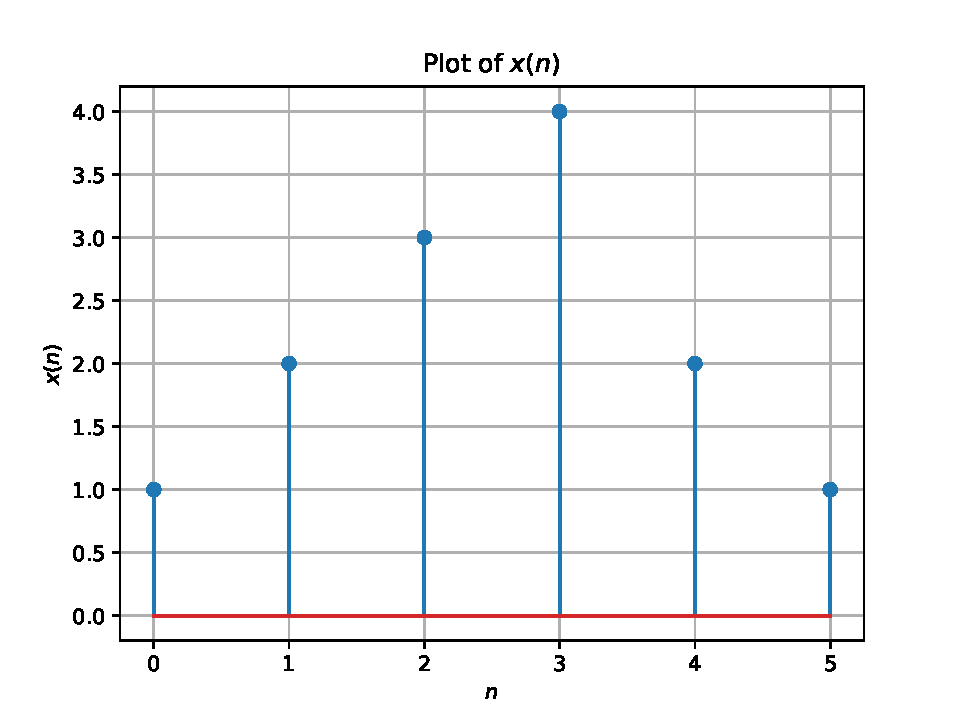
\includegraphics[width=\columnwidth]{Figure_1.pdf}
\end{center}
\captionof{figure}{}
\label{fig:1}	
\end{figure}


\item Let
\begin{multline}
\label{eq:iir_filter}
y(n) + \frac{1}{2}y(n-1) = x(n) + x(n-2), 
\\
 y(n) = 0, n < 0
\end{multline}
Sketch $y(n)$.  
\\
\solution The Python code for sketching the graph of $y(n)$ can be found in the link below. The code yields the graph shown in figure \ref{fig:2}
\begin{lstlisting}
wget https://github.com/anitadash/EE3900/blob/main/Codes/3_2.py
\end{lstlisting}
\begin{figure}[!ht]
\begin{center}
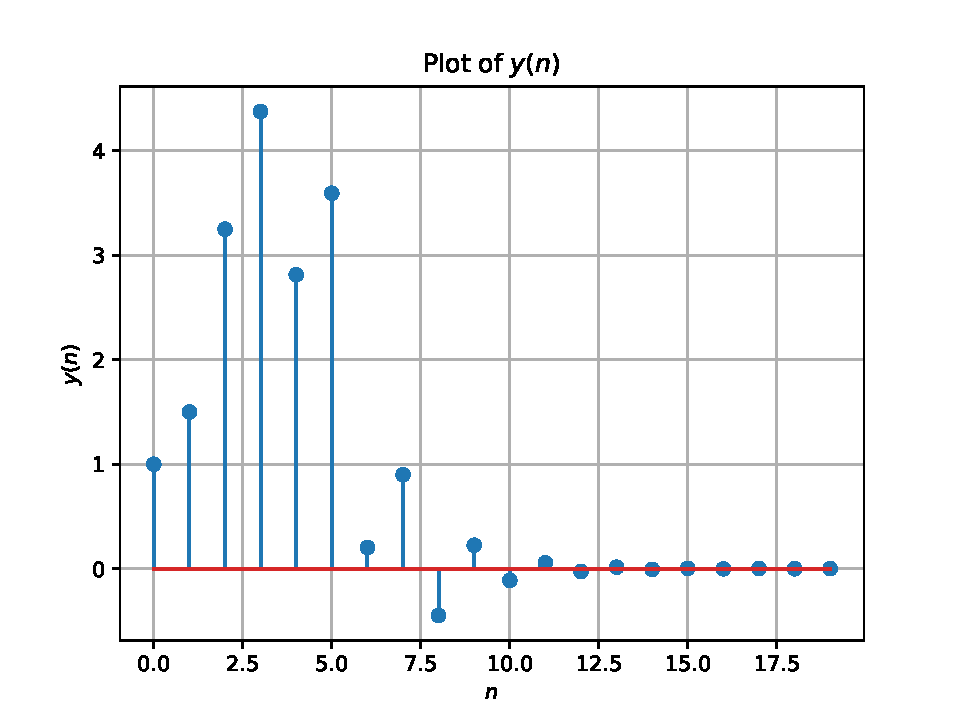
\includegraphics[width=\columnwidth]{Figure_2.pdf}
\end{center}
\captionof{figure}{}
\label{fig:2}	
\end{figure}


\item Repeat the above exercise using a C code.
\\
\solution The C-code for the above two exercises can be found in the link below. The code yields the graph shown in figure \ref{fig:6}
\begin{lstlisting}
wget https://github.com/anitadash/EE3900/blob/main/Codes/3_3.c
\end{lstlisting}
\begin{figure}[!ht]
\begin{center}
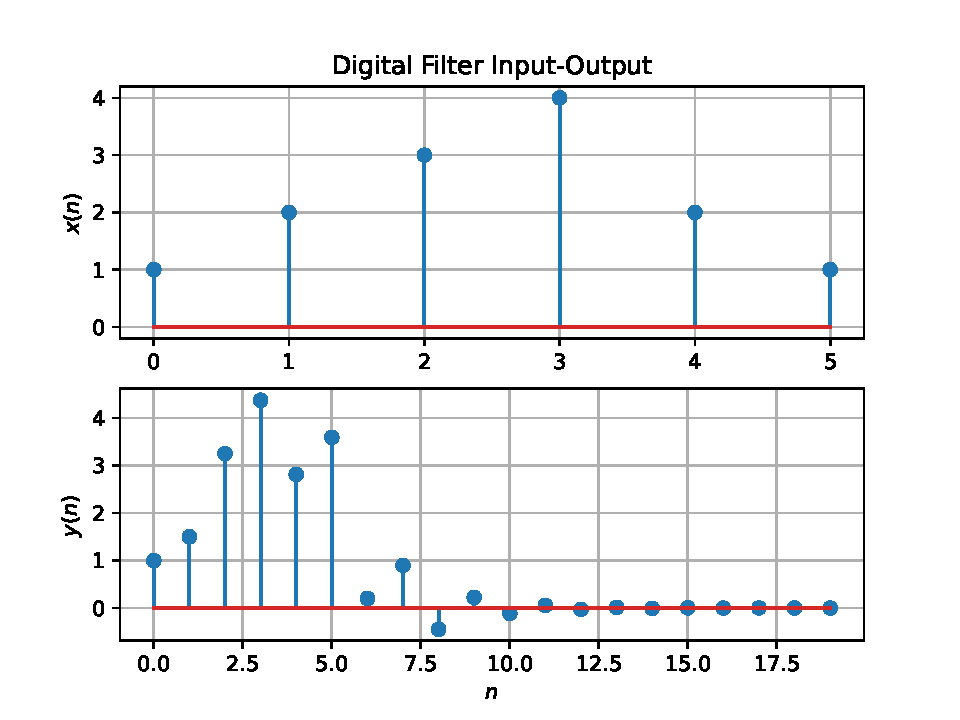
\includegraphics[width=\columnwidth]{Figure_6.pdf}
\end{center}
\captionof{figure}{}
\label{fig:6}	
\end{figure}
\end{enumerate}


\section{Z-transform}
\begin{enumerate}[label=\thesection.\arabic*
,ref=\thesection.\theenumi]

\item The $Z$-transform of $x(n)$ is defined as
%
\begin{equation}
\label{eq:z_trans}
X(z)={\mathcal {Z}}\{x(n)\}=\sum _{n=-\infty }^{\infty }x(n)z^{-n}
\end{equation}
%
Show that
\begin{equation}
\label{eq:shift1}
{\mathcal {Z}}\{x(n-1)\} = z^{-1}X(z)
\end{equation}
and find
\begin{equation}
	{\mathcal {Z}}\{x(n-k)\} 
\end{equation}
\solution From \eqref{eq:z_trans},
\begin{align}
{\mathcal {Z}}\{x(n-1)\} &=\sum _{n=-\infty }^{\infty }x(n-1)z^{-n}
\\
&=\sum _{n=-\infty }^{\infty }x(n)z^{-n-1} = z^{-1}\sum _{n=-\infty }^{\infty }x(n)z^{-n}
\end{align}
Similarly,
\begin{align}
{\mathcal {Z}}\{x(n-k)\} &=\sum _{n=-\infty }^{\infty }x(n-k)z^{-n}
\\
&=\sum _{n=-\infty }^{\infty }x(n)z^{-n-k} = z^{-k}\sum _{n=-\infty }^{\infty }x(n)z^{-n}
\end{align}
Therefore,
\begin{equation}
\label{eq:shiftk}
{\mathcal {Z}}\{x(n-k)\} = z^{-k}X(z)
\end{equation}


\item Obtain $X(z)$ for $x(n)$ defined in problem 
	\ref{eq:x}.
\\
\solution We Know that,
\begin{align}
X(z)&=\sum _{n=-\infty }^{\infty }x(n)z^{-n}
\\
\implies X(z)&= \sum _{n=0}^{5}x(n)z^{-n}
\end{align}
Therefore,
\begin{equation}
    X(z)= 1 + \frac{2}{z} + \frac{3}{z^{2}} + \frac{4}{z^{3}} + \frac{2}{z^{4}} + \frac{1}{z^{5}} 
\end{equation}


\item Find
%
\begin{equation}
H(z) = \frac{Y(z)}{X(z)}
\end{equation}
%
from  \eqref{eq:iir_filter} assuming that the $Z$-transform is a linear operation.
\\
\solution from  \eqref{eq:iir_filter} assuming that the $Z$-transform is a linear operation.
\\
Applying \eqref{eq:shiftk} in \eqref{eq:iir_filter} we get,
\begin{align}
Y(z) + \frac{1}{2}z^{-1}Y(z) &= X(z)+z^{-2}X(z)
\\
\implies \frac{Y(z)}{X(z)} &= \frac{1 + z^{-2}}{1 + \frac{1}{2}z^{-1}}
\label{eq:freq_resp}
\end{align}


\item Find the Z transform of 
\begin{equation}
\delta(n)
=
\begin{cases}
1 & n = 0
\\
0 & \text{otherwise}
\end{cases}
\end{equation}
and show that the $Z$-transform of
\begin{equation}
\label{eq:unit_step}
u(n)
=
\begin{cases}
1 & n \ge 0
\\
0 & \text{otherwise}
\end{cases}
\end{equation}
is
\begin{equation}
U(z) = \frac{1}{1-z^{-1}}, \quad |z|>1
\end{equation}
\\
\solution From \eqref{eq:z_trans}, we can see that,
\begin{equation}
{\mathcal {Z}}\{\delta(n)\} = \delta(0)z^{0}
\implies {\mathcal {Z}}\{\delta(n)\} = 1
\end{equation}
To show that the $Z$-transform of $u(n)$ is
\begin{equation}
U(z) = \frac{1}{1-z^{-1}}, \quad |z|>1
\end{equation}
From \eqref{eq:z_trans}, we can see that,
\begin{align}
{\mathcal {Z}}\{u(n)\} &=\sum _{n=0}^{\infty }u(n)z^{-n}
\\
&=\sum _{n=0}^{\infty }z^{-n}
\end{align}
The above summation is an infinite geometric progression with common ratio $z^{-1}$, and for an infinite geometric progression to converge the common ratio must be strictly lesser than 1.
\\
Therefore
\begin{equation}
    U(z) = \frac{1}{1-z^{-1}}, \quad |z|>1
\end{equation}


\item Show that,
\begin{equation}
\label{eq:anun}
    a^nu(n) \ztrans \frac{1}{1-az^{-1}} \quad |z| > |a|
\end{equation}
\solution From \eqref{eq:unit_step} we can see that,
\begin{equation}
    {\mathcal {Z}}\{a^{n}u(n)\} =\sum _{n=0}^{\infty }a^{n}z^{-n}
\end{equation}
The above summation is an infinite geometric progression with common ratio $az^{-1}$, and for an infinite geometric progression to converge the common ratio must be strictly lesser than 1. (Which is true as given $|z|>|a|$)
\\
Therefore the $Z$-tranform of $a^{n}u{n}$ is,
\begin{equation}
    a^nu(n) \ztrans \frac{1}{1-az^{-1}} \quad |z| > |a|
\end{equation}


\item
Let
\begin{equation}
H\brak{e^{j \omega}} = H\brak{z = e^{j \omega}}.
\end{equation}
Plot $|H\brak{e^{j \omega}}|$.  Is it periodic? If so, find the period. $H(e^{j \omega})$ is
known as the {\em Discret Time Fourier Transform} (DTFT) of $h(n)$.
\\
\solution The Python code for sketching the graph of $H\brak{e^{j\omega}}$ can be found in the link below. The above code yields figure \ref{fig:3}.
\begin{lstlisting}
wget https://github.com/anitadash/EE3900/blob/main/Codes/4_5.py
\end{lstlisting}                
\begin{figure}[!ht]
\begin{center}
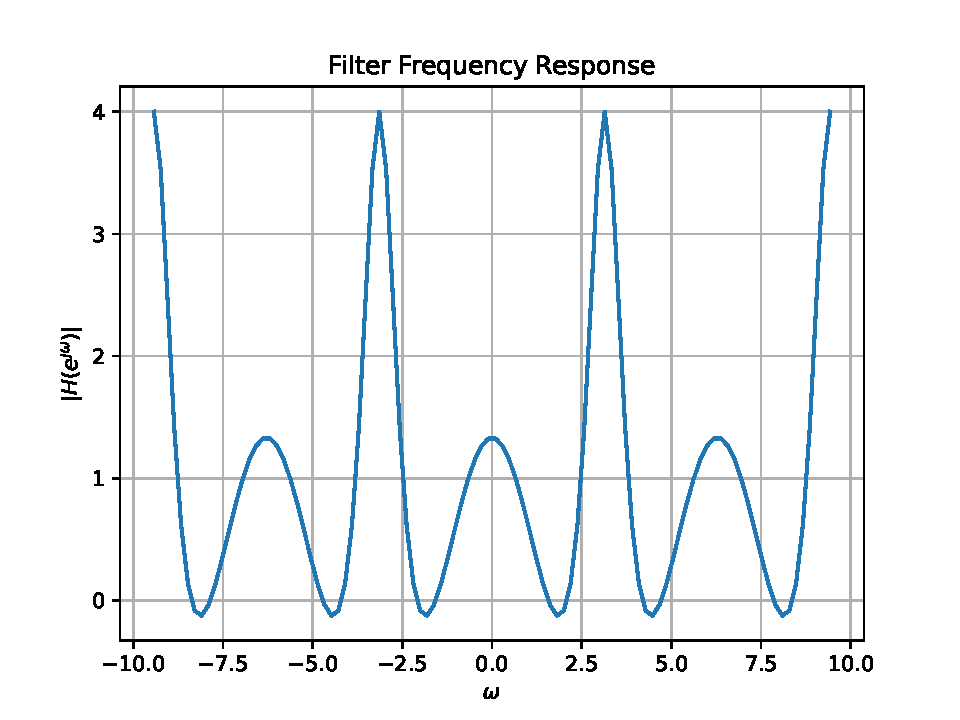
\includegraphics[width=\columnwidth]{Figure_3.pdf}
\end{center}
\captionof{figure}{}
\label{fig:3}	
\end{figure}
It is periodic with a period of $2\pi$.\\
Proof:
\begin{align}
H\brak{e^{j (\omega+2\pi)}} = H\brak{e^{j \omega}e^{j2\pi}}\\
=H\brak{e^{j \omega}(\cos(2\pi)+j\sin(2\pi))}\\
=H\brak{e^{j \omega}}
\end{align}
$2\pi$ is a period, we need to verify whether if it is the fundamental period.and thus need to check the periodicity for $T=\pi$\\
\begin{align}
H\brak{e^{j (\omega+\pi)}}=-H\brak{e^{j \omega}}       
\end{align}
and thus $2\pi$ is the period of the function.
\item Express $h(n)$ in terms of $H\brak{e^{j \omega}}$.
\\
\solution $h(n)$ can be expressed as:
\begin{equation}
\label{eq:idft}
h(n) = \frac{1}{2\pi} \int_{0}^{2\pi} H\brak{e^{\j \omega}}e^{\j n \omega}d \omega
\end{equation}
Proof: We know that\\
\begin{equation}
H\brak{e^{\j \omega}} = \sum _{k=0}^{\infty }h(k)z^{-\j k \omega}
\end{equation}
Substituting the above equation in \eqref{eq:idft}
\begin{align}
h(n) = \frac{1}{2\pi}\int_{0}^{2\pi}\brak{ \sum _{k=0}^{\infty }h(k)z^{-\j k \omega}}e^{\j n \omega}d \omega\\
h(n) = \frac{1}{2\pi}\sum _{k=0}^{\infty }h(k)\int_{0}^{2\pi}z^{\j(n-k) \omega}d \omega
\end{align}
The above integral is $1$ when $k=n$ and $0$ otherwise. Thus,
\begin{equation}
h(n) = \frac{1}{2\pi}\int_{0}^{2\pi} H\brak{e^{\j \omega}}e^{\j n \omega}d \omega
\end{equation}
Hence Shown.
\end{enumerate}



\section{Impulse Response}
\begin{enumerate}[label=\thesection.\arabic*]
\item Using long division, 
find
		\begin{align}
			h(n), \quad n < 5
		\end{align}
		for H(z) in 
		\eqref{eq:freq_resp}.
\\
\solution Given,
\begin{align}
     H(z) = \frac{1 + z^{-2}}{1 + \frac{1}{2}z^{-1}}
     \\
     H(z) = \frac{2z^{2}+2}{2z^{2}+z}
\end{align}
By Long Division, $H(z)=$
\begin{align}
    \begin{array}{r}
         1-\frac{1}{2z}+\frac{5}{4z^2}-\frac{5}{8z^3}\ldots  \\
         2z^2+z{\overline{\smash{\big)}\,2z^2 + 2\phantom{)}}}\\
         \underline{-~\phantom{(}(2z^2 + z)\phantom{)}}\\
         -z + 2\phantom{)}\\ 
        \underline{-~\phantom{()}(-z-\frac{1}{2})}\\ 
        \frac{5}{2}\phantom{)} \\
        \underline{-~\phantom{(}(\frac{5}{2} + \frac{5}{4z})\phantom{)}}\\
        \frac{-5}{4z}\phantom{)}\\
        \underline{-~\phantom{(}(\frac{-5}{4z} + \frac{-5}{8z^2})\phantom{)}}\\
        \frac{-5}{8z^2}\phantom{)}\\
        \vdots\phantom{)}
    \end{array}
\end{align}
From the above we can see that 
\begin{equation}
\label{eq:H}
    H(z) = 1 - \frac{1}{2z} + \frac{5}{4z^{2}} - \frac{5}{8z^{3}} + \ldots 5\brak{\frac{-1}{2z}}^{n} (n>1)
\end{equation}
given n $<$ 5 , Therefore 
\begin{equation}
    H(z) = \sum _{n=-\infty }^{4}h(n)z^{-n}
\end{equation}
Therefore, comparing the above equation with \eqref{eq:H} we can say that,
\begin{equation}
    h(n) = \cbrak{1,\frac{-1}{2},\frac{5}{4},\frac{-5}{8},\frac{5}{16}}
\end{equation}


\item \label{prob:impulse_resp}
Find an expression for $h(n)$ using $H(z)$, given that 
%in Problem \ref{eq:ztransab} and \eqref{eq:anun}, given that
\begin{equation}
\label{eq:impulse_resp}
h(n) \ztrans H(z)
\end{equation}
and there is a one to one relationship between $h(n)$ and $H(z)$. $h(n)$ is known as the {\em impulse response} of the
system defined by \eqref{eq:iir_filter}.
\\
\solution Given,
\begin{equation}
\label{eq:impulse_resp}
h(n) \ztrans H(z)
\end{equation}
We know that,
\begin{align}
    H(z) &= \frac{1 + z^{-2}}{1 + \frac{1}{2}z^{-1}}
    \\
    &= \frac{1}{1 + \frac{1}{2}z^{-1}} + \frac{z^{-2}}{1 + \frac{1}{2}z^{-1}}    
\end{align}
From \eqref{eq:anun} and \eqref{eq:shiftk}, we can say that
\begin{equation}
    h(n) = \brak{-\frac{1}{2}}^{n}u(n) + \brak{-\frac{1}{2}}^{n-2}u(n-2) 
\end{equation}


\item Sketch $h(n)$. Is it bounded? Justify theoretically.
\\
\solution The Python code for sketching the graph of $h(n)$ can be found in the link below. The above code yields the graph shown in figure \ref{fig:4}
\begin{lstlisting}
wget https://github.com/anitadash/EE3900/blob/main/Codes/5_2.py
\end{lstlisting}
We know that,
\begin{equation}
    0 \le u(n) \le 1  \quad \forall n \ge 0    
\end{equation}
\begin{equation}
\label{eq:a}
    0 \le \brak{\frac{-1}{2}}^{n}u(n) \le \brak{\frac{-1}{2}}^{n} \le 1  \quad \forall n \ge 0
\end{equation}
Similarly,
\begin{equation}
\label{eq:b}
    0 \le \brak{\frac{-1}{2}}^{n-2}u(n-2)\le \brak{\frac{-1}{2}}^{n-2} \le 1  \quad \forall n \ge 0
\end{equation}
Adding \eqref{eq:a} and \eqref{eq:b}, We get
\begin{equation}
    0 \le h(n) \le 2  \quad \forall n \ge 0
\end{equation}
Thus, $h(n)$ is bounded.
\begin{figure}[!ht]
\begin{center}
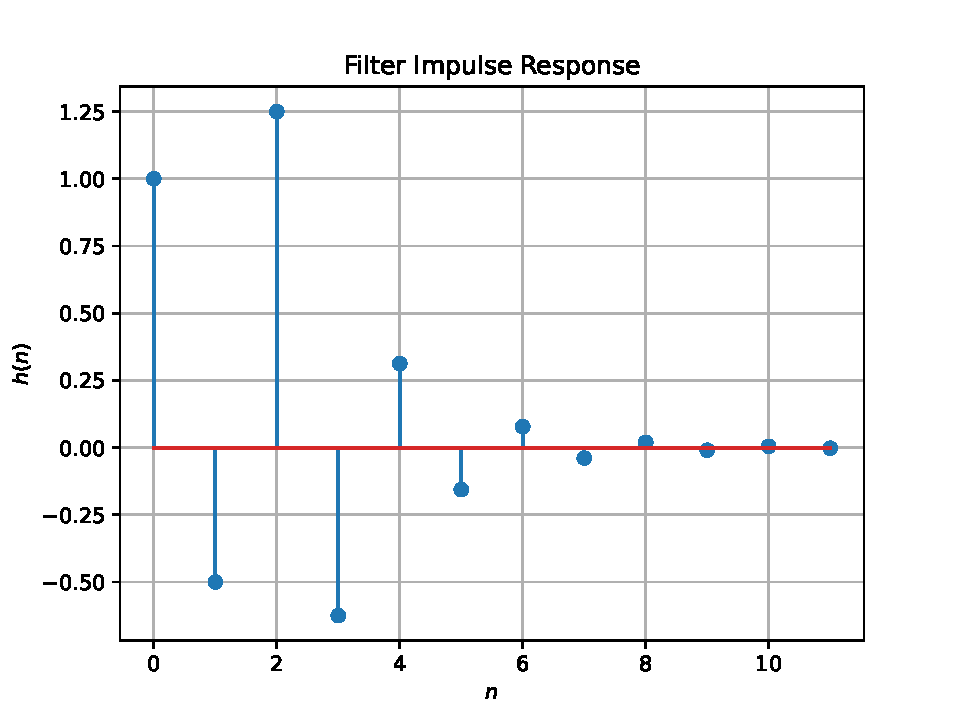
\includegraphics[width=\columnwidth]{Figure_4.pdf}
\end{center}
\captionof{figure}{}
\label{fig:4}	
\end{figure}


\item Convergent? Justify using the ratio test.
\\
\solution from \eqref{eq:H} We can see that for $n>1$ 
\begin{equation}
h(n) = 5\brak{\frac{-1}{2}}^n
\end{equation}
Ratio test states that:\\
If $a(n)$ is a sequence such that
\begin{equation}
\lim_{n \to+\infty}|\frac{a_{n+1}}{a_{n}}| = L
\end{equation}
and if $L<1$ , then $a(n)$ converges. Thus,
\begin{align}
\lim_{n \to+\infty}|\frac{h_{n+1}}{h_{n}}| = \frac{5\brak{\frac{1}{2}}^{n+1}}{5\brak{\frac{1}{2}}^n}
&= \frac{1}{2}
\end{align}
Hence, $h(n)$ is convergent.


\item The system with $h(n)$ is defined to be stable if
\begin{equation}
\sum_{n=-\infty}^{\infty}h(n) < \infty
\end{equation}
Is the system defined by \eqref{eq:iir_filter} stable for the impulse response in \eqref{eq:impulse_resp}?
\\
\solution
We know that,
\begin{equation}
    h(n) = \brak{-\frac{1}{2}}^{n}u(n) + \brak{-\frac{1}{2}}^{n-2}u(n-2)
\end{equation}
\begin{align}
\sum_{n=-\infty}^{\infty}h(n)&=\sum_{n=0}^{\infty}\brak{-\frac{1}{2}}^{n}+\sum_{n=2}^{\infty}\brak{-\frac{1}{2}}^{n-2}
\\
&= \brak{\frac{1}{1+\frac{1}{2}}} + \brak{\frac{1}{1+\frac{1}{2}}}
\\
&=\frac{4}{3}
\end{align}
Therefore,
\begin{equation}
\sum_{n=-\infty}^{\infty}h(n) < \infty
\end{equation}
Hence the system defined by \eqref{eq:iir_filter} is stable for the impulse response in \eqref{eq:impulse_resp}


\item Verify the above result using a python code.
\solution The python code to the question can be found in the link below
\begin{lstlisting}
wget https://github.com/anitadash/EE3900/blob/main/Codes/5_6.py
\end{lstlisting}


\item 
Compute and sketch $h(n)$ using 
\begin{equation}
\label{eq:iir_filter_h}
h(n) + \frac{1}{2}h(n-1) = \delta(n) + \delta(n-2), 
\end{equation}
%
This is the definition of $h(n)$.
\\
\solution The Python code for sketching the graph of $h(n)$ from \eqref{eq:iir_filter_h} can be found in the link below. The code yields the graph shown in figure \ref{fig:5}
\begin{lstlisting}
wget https://github.com/anitadash/EE3900/blob/main/Codes/5_4.py
\end{lstlisting}
\begin{figure}[!ht]
\begin{center}
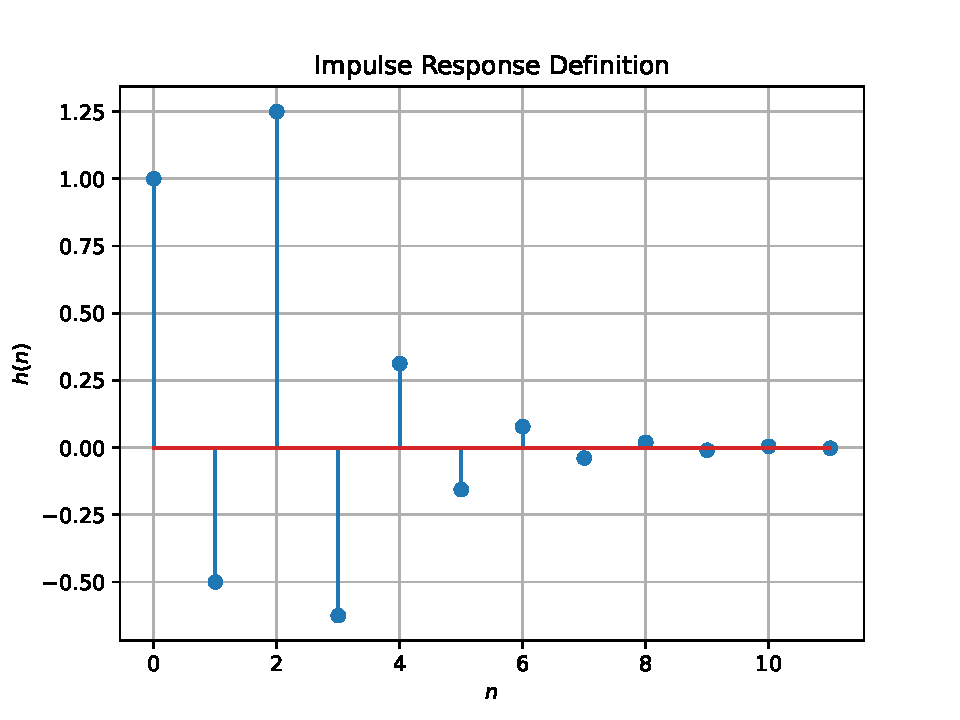
\includegraphics[width=\columnwidth]{Figure_5.pdf}
\end{center}
\captionof{figure}{}
\label{fig:5}	
\end{figure}  
\item Compute 
%
\begin{equation}
\label{eq:convolution}
y(n) = x(n)*h(n) = \sum_{n=-\infty}^{\infty}x(k)h(n-k)
\end{equation}
%
Comment. The operation in \eqref{eq:convolution} is known as
{\em convolution}.
%
\\
\solution The Python code for the question can be found in the link below. The code yields the graph shown in figure \ref{fig:7}. $y(n)$ is the same as the $y(n)$ from \eqref{eq:iir_filter}
\begin{lstlisting}
wget https://github.com/anitadash/EE3900/blob/main/Codes/5_8.py
\end{lstlisting}
\begin{figure}[!ht]
\begin{center}
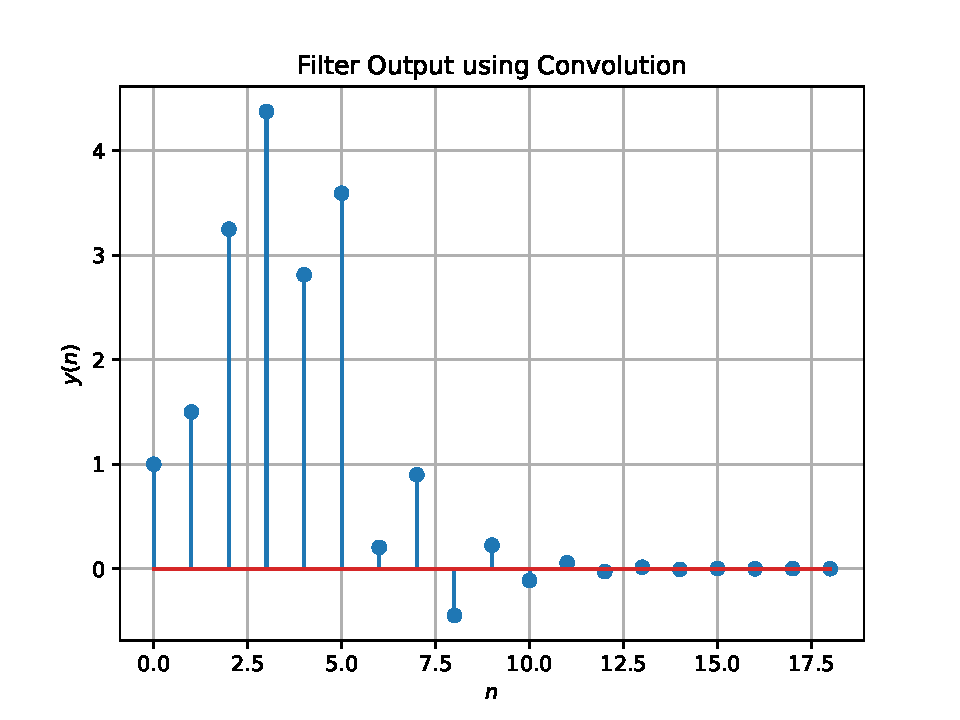
\includegraphics[width=\columnwidth]{Figure_7.pdf}
\end{center}
\captionof{figure}{}
\label{fig:7}	
\end{figure}  
    

\item Express the above convolution using a Teoplitz matrix.\\
\solution following is the Teoplitz matrix $T$ \\ \\
$\begin{smallmatrix}
1 & 0 & 0 & 0 & 0 & 0\\
-5 & 1 & 0 & 0 & 0 & 0\\
1.25 &-5 & 1 & 0 & 0 & 0\\
-0.62 & 1.25 & -5 & 1 & 0 & 0\\
0.31 & -0.62 & 1.25 & -5 & 1 & 0\\
-0.16 & 0.31 & -0.62 & 1.25 & -5 & 1\\
0.08 & -0.16 & 0.31 & -0.62 & 1.25 & -5\\
-0.04 & 0.08 & -0.16 & 0.31 & -0.62 & 1.25\\
0.02 & -0.04 & 0.08 & -0.16 & 0.31 & 0.62\\
-9.76e^{-3} & 0.02 & -0.04 & 0.08 & -0.16 & 0.31 \\
4.88e^{-3} & -9.76e^{-3} & 0.02 & -0.04 & 0.08 & -0.16\\
-2.44e^{-3} & 4.88e^{-3} & -9.76e^{-3} & 0.02 & -0.04 & 0.08\\
1.22e^{-3} & -2.44e^{-3} & 4.88e^{-3} & -9.76e^{-3} & 0.02 & -0.04\\
-6.1e^{-4} & 1.22e^{-3} & -2.44e^{-3} & 4.88e^{-3} & -9.76e^{-3} & 0.02\\
0 & -6.1e^{-4} & 1.22e^{-3} & -2.44e^{-3} & 4.88e^{-3} & -9.76e^{-3}\\
0 & 0 & -6.1e^{-4} & 1.22x10^{-3} & -2.44e^{-3} & 4.88e^{-3}\\
0 & 0 & 0 & -6.1e^{-4} & 1.22e^{-3} & -2.44e^{-3}\\
0 & 0 & 0 & 0 & -6.1e^{-4} & 1.22e^{-3}\\
0 & 0 & 0 & 0 & 0 & -6.1e^{-4}
\end{smallmatrix}$ 
\\ \\
Therefore $T.X$ gives,
\begin{align}
y = 
\begin{bmatrix}
  1\\
  1.5 \\
  3.25\\
  4.375\\
  2.81 \\
  3.59 \\
  0.203 \\
  0.89\\
 -0.449 \\
  0.224\\
 -0.11 \\
  5.61e^{-2}\\
 -2.80e^{-2} \\ 
 1.40e^{-2} \\
 -7.01e^{-3} \\
 3.50e^{-3}\\
 -1.75e^{-3} \\ 
 8.77e^{-4} \\
 -4.38e^{-4} \\
 0\\
\end{bmatrix}
\end{align}
\item Show that
\begin{equation}
y(n) =  \sum_{n=-\infty}^{\infty}x(n-k)h(k)
\end{equation}

\solution We know that,
\begin{equation}
Y(z) = H(z).X(z)
\end{equation}
Therefore,
\begin{equation}
\sum_{n=-\infty}^{\infty}y(n)z^{-n} = \sum_{n=-\infty}^{\infty}h(n)z^{-n}\sum_{n=-\infty}^{\infty}x(n)z^{-n}
\end{equation}
\begin{align}
=\sum_{n=-\infty}^{\infty}\sum_{k=0}^{n}h(k)x(n-k)z^{-n}
\end{align}
Therefore, By comparison we can see that,
\begin{equation}
y(n) = \sum_{k=0}^{n}h(k)x(n-k)
\end{equation}
\end{enumerate}   


\section{DFT}
\begin{enumerate}[label=\thesection.\arabic*
,ref=\thesection.\theenumi]
\item
Compute
\begin{equation}
X(k) \define \sum _{n=0}^{N-1}x(n) e^{-\j2\pi kn/N}, \quad k = 0,1,\dots, N-1
\end{equation}
and $H(k)$ using $h(n)$.\\
\solution We know that,
\begin{equation}
x(n) = \cbrak{1,2,3,4,2,1}
\end{equation}
Adding and subtracting $e^{-j2\pi k6/6}$ we get,
\begin{equation}
X(k) = \sum _{n=0}^{6}x(n) e^{-\j2\pi kn/N} - 1
\end{equation}
\begin{align}
\frac{2\pi kn}{6} + \frac{2\pi kn}{6}
\end{align}
\item Compute 
\begin{equation}
Y(k) = X(k)H(k)
\end{equation}
\solution We know that,
\begin{align}
X(k) = \sum _{n=0}^{N-1}x(n) e^{-\j2\pi kn/N}\\
H(k) = \sum _{n=0}^{N-1}h(n) e^{-\j2\pi kn/N}
\end{align}
\begin{equation}
X(k)H(k)= \sum _{n=0}^{N-1}\brak{x(n)*h(n)} e^{-\j2\pi kn/N}
\end{equation}
\begin{align}
\implies \sum _{n=0}^{N-1}y(n) e^{-\j2\pi kn/N}
\end{align}
therefore, 
\begin{equation}
Y(k) = X(k)H(k)
\end{equation}
\item Compute
\begin{equation}
 y\brak{n}={\frac {1}{N}}\sum _{k=0}^{N-1}Y\brak{k}\cdot e^{\j 2\pi kn/N},\quad n = 0,1,\dots, N-1
\end{equation}
\solution The Python code for the computation can be found below . The code yields the graph shown in figure \ref{fig:8}
\begin{lstlisting}
wget https://github.com/anitadash/EE3900/blob/main/Codes/6_3.py
\end{lstlisting}
\begin{figure}[!ht]
\begin{center}
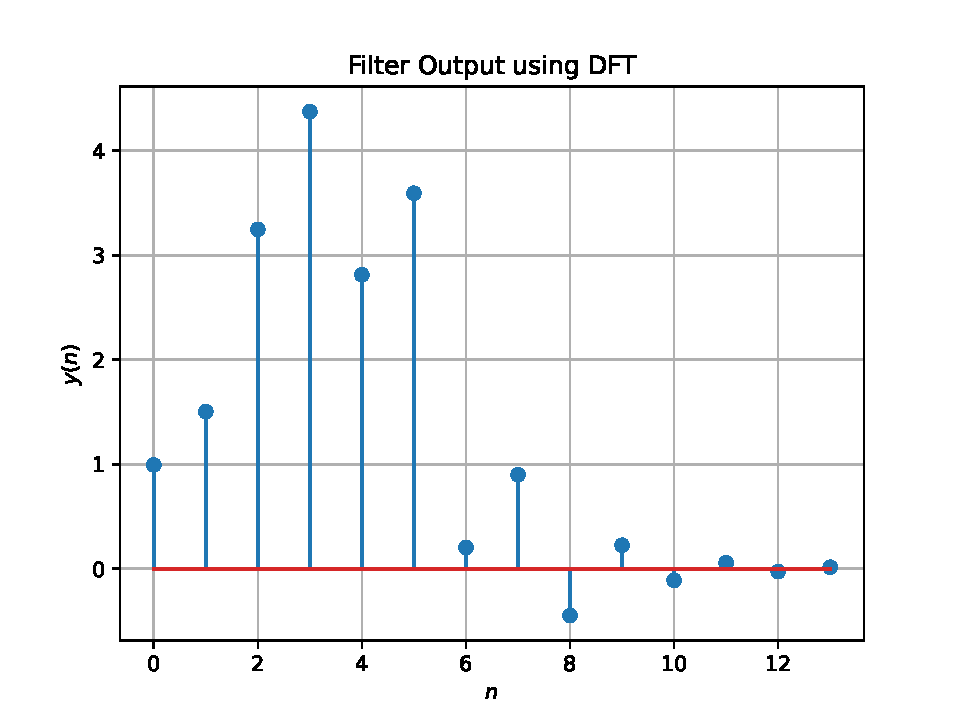
\includegraphics[width=\columnwidth]{Figure_8.pdf}
\end{center}
\captionof{figure}{}
\label{fig:8}	
\end{figure}  
\item Repeat the previous exercise by computing $X(k), H(k)$ and $y(n)$ through FFT and 
IFFT.
\solution The Python code for the computation can be found below.
\begin{lstlisting}
wget https://github.com/anitadash/EE3900/blob/main/Codes/6_4.py
\end{lstlisting}
\begin{figure}[!ht]
\begin{center}
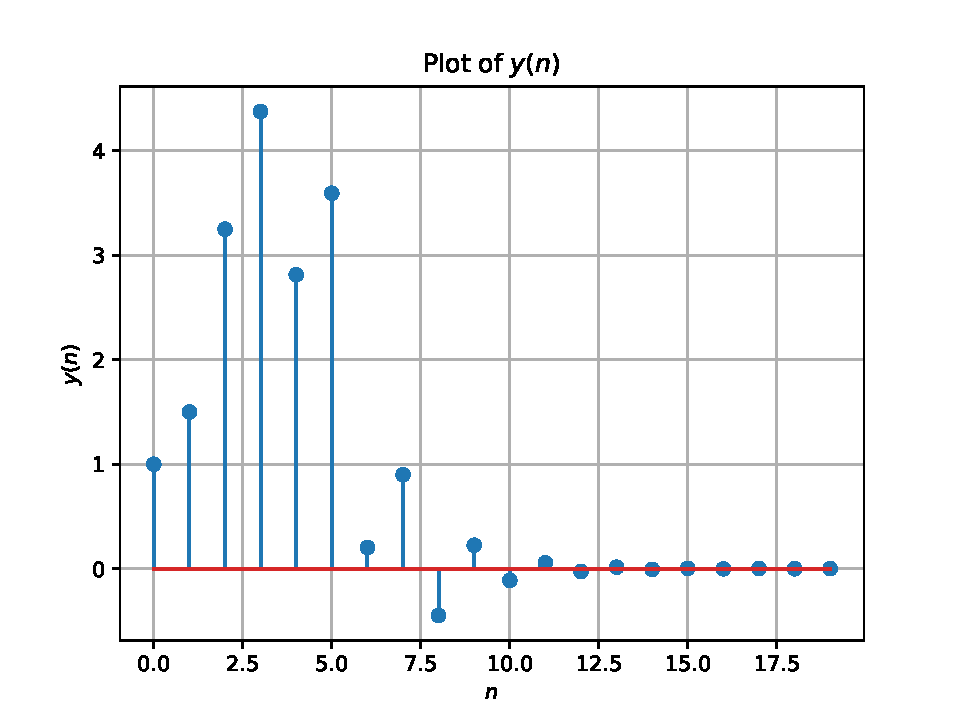
\includegraphics[width=\columnwidth]{Figure_2.pdf}
\end{center}
\captionof{figure}{}
\label{fig:9}	
\end{figure}
\begin{figure}[!ht]
\begin{center}
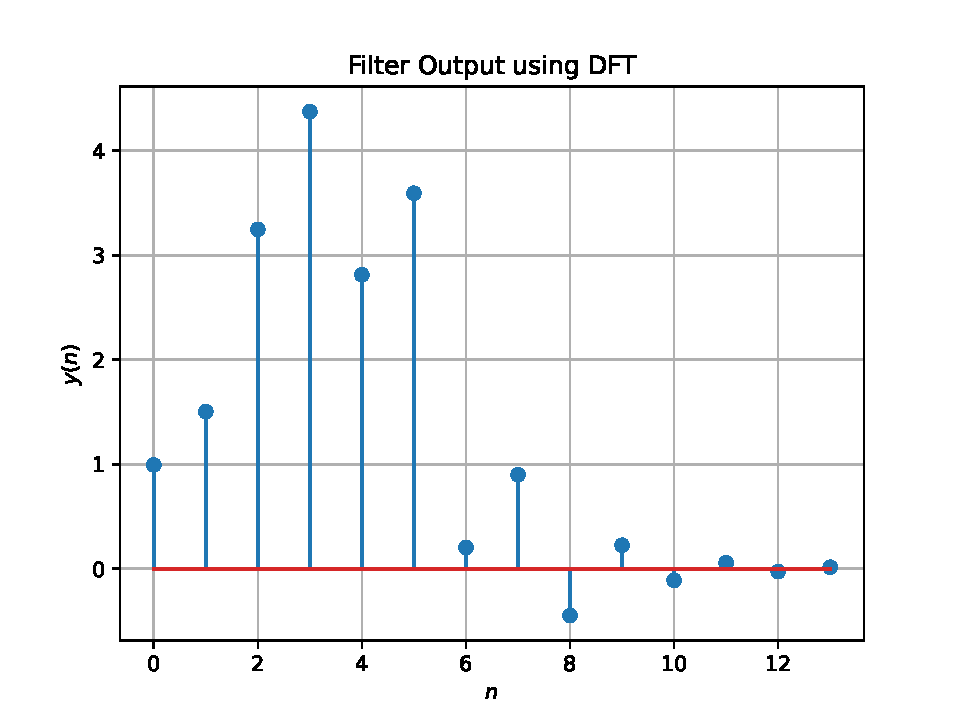
\includegraphics[width=\columnwidth]{Figure_8.pdf}
\end{center}
\captionof{figure}{}
\label{fig:10}	
\end{figure}
\begin{figure}[!ht]
\begin{center}
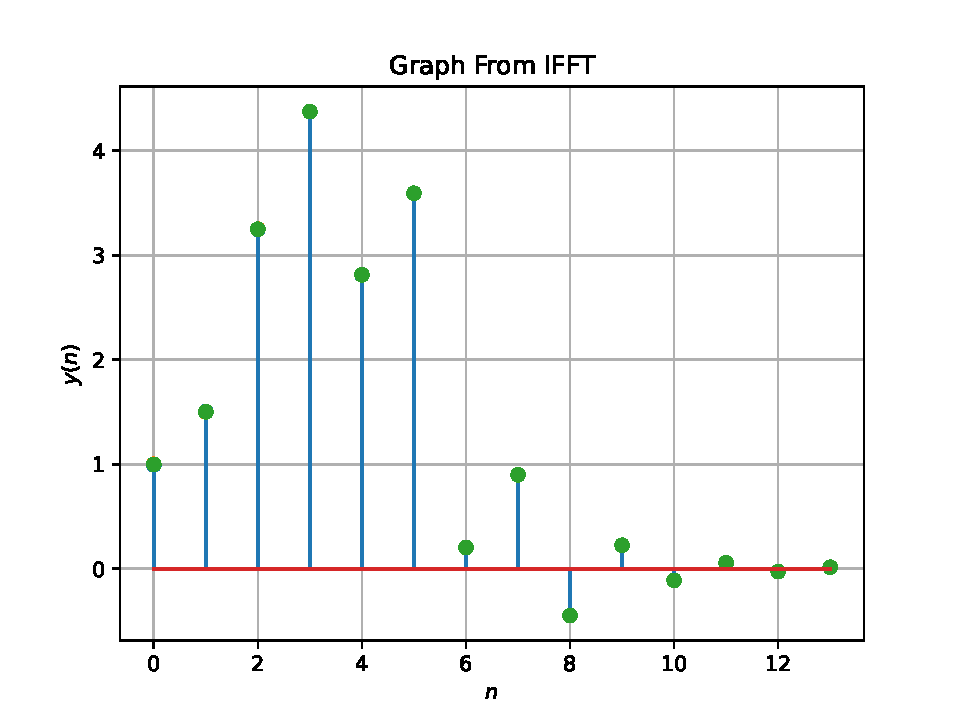
\includegraphics[width=\columnwidth]{Figure_10.pdf}
\end{center}
\captionof{figure}{}
\label{fig:11}	
\end{figure}
\end{enumerate}

\section{FFT}
\begin{enumerate}[label=\thesection.\arabic*]

\numberwithin{equation}{section}
    \item The DFT of $x(n)$ is given by
    \begin{align}
        X(k) \triangleq \sum_{n=0}^{N-1} x(n) e^{-j 2 \pi k n / N}, \quad k=0,1, \ldots, N-1
    \end{align}
\item Let 
	\begin{align}
W_{N} = e^{-j2\pi/N} 
	\end{align}
		Then the $N$-point {\em DFT matrix} is defined as 
	\begin{align}
		\vec{F}_{N} = \sbrak{W_{N}^{mn}}, \quad 0 \le m,n \le N-1 
	\end{align}
	where $W_{N}^{mn}$ are the elements of $\vec{F}_{N}$.
\item Let 
	\begin{align}
		\vec{I}_4 = \myvec{\vec{e}_4^{1} &\vec{e}_4^{2} &\vec{e}_4^{3} &\vec{e}_4^{4} }
	\end{align}
		be the $4\times 4$ identity matrix.  Then the 4 point {\em DFT permutation matrix} is defined as 
	\begin{align}
		\vec{P}_4 = \myvec{\vec{e}_4^{1} &\vec{e}_4^{3} &\vec{e}_4^{2} &\vec{e}_4^{4} }
	\end{align}
\item The 4 point {\em DFT diagonal matrix} is defined as 
	\begin{align}
		\vec{D}_4 = diag\myvec{W_{8}^{0} & W_{8}^{1} & W_{8}^{2} & W_{8}^{3}}
	\end{align}
\item Show that 
\begin{equation}
    W_{N}^{2}=W_{N/2}
\end{equation} 
\solution We know that,
\begin{align}
W_{N}^{2} = \brak{e^{\frac{-j2\pi}{N}}}^{2}
= e^{\frac{-j2\pi}{N/2}}
= W_{N/2}
\end{align}
therefore,
\begin{equation}
    W_{N}^{2}=W_{N/2}
\end{equation} 
\item Show that 
\begin{equation}
	\vec{F}_{4}=
\begin{bmatrix}
	\vec{I}_{2} & \vec{D}_{2} \\
\vec{I}_{2} & -\vec{D}_{2}
\end{bmatrix}
\begin{bmatrix}
\vec{F}_{2} & 0 \\
0 & \vec{F}_{2}
\end{bmatrix}
\vec{P}_{4}
\label{eq:fft-recurrence}
\end{equation}
\solution We know that for $n \in \mathbb{N}$,
\begin{align}
W_4^{4n} = 1 \\
W_4^{4n + 2} = -1
\end{align}
Thus,
\begin{align}
	\vec{D}_2\vec{F}_2 &= \mybvec{\w{4}{0} & 0 \\ 0 & \w{4}{1}}\mybvec{\w{2}{0} & \w{2}{0} \\ \w{2}{0} & \w{2}{1}} \\
					   &= \mybvec{\w{4}{0} & 0 \\ 0 & \w{4}{1}}\mybvec{\w{4}{0} & \w{4}{0} \\ \w{4}{0} & \w{4}{2}} \\
					   &= \mybvec{\w{4}{0} & \w{4}{0} \\ \w{4}{1} & \w{4}{3}} \label{eq:fft-df1} \\
	\implies -\vec{D}_2\vec{F}_2 &= \mybvec{\w{4}{2} & \w{4}{6} \\ \w{4}{3} & \w{4}{9}} \label{eq:fft-df2}
\end{align}
and
\begin{align}
	\vec{F}_2 &= \myvec{\w{2}{0} & \w{2}{0} \\ \w{2}{0} & \w{2}{1}} \\
			  &= \myvec{\w{4}{0} & \w{4}{0} \\ \w{4}{0} & \w{4}{2}}
\end{align}
Hence,
\begin{align}
	\vec{W}_4 &= \myvec{\w{4}{0} & \w{4}{0} & \w{4}{0} & \w{4}{0} \\
		\w{4}{0} & \w{4}{2} & \w{4}{1} & \w{4}{3} \\
		\w{4}{0} & \w{4}{4} & \w{4}{2} & \w{4}{6} \\
		\w{4}{0} & \w{4}{6} & \w{4}{3} & \w{4}{9} 
	} \label{eq:fft-permutation} \\
	&= \mybvec{\vec{I}_2\vec{F}_2 & \vec{D}_2{F}_2 \\ \vec{I}_2\vec{F}_2 & -\vec{D}_2{F}_2} \\
	&= \mybvec{\vec{I}_2 & \vec{D}_2 \\ \vec{I}_2 & \vec{D}_2}\mybvec{\vec{F}_2 & 0 \\ 0 & \vec{F}_2}
	\label{eq:ifd}
\end{align}
Multiplying \eqref{eq:ifd} by $\vec{P}_4$ on both sides, and noting that $\vec{W}_4\vec{P}_4 = \vec{F}_4$ gives us \eqref{eq:fft-recurrence}.
\item Show that 
\begin{equation}
\vec{F}_{N}=
\begin{bmatrix}
\vec{I}_{N/2} & \vec{D}_{N/2} \\
\vec{I}_{N/2} & -\vec{D}_{N/2}
\end{bmatrix}
\begin{bmatrix}
\vec{F}_{N/2} & 0 \\
0 & \vec{F}_{N/2}
\end{bmatrix}
\vec{P}_{N}
\end{equation}
\solution Observe that for even $N$ and letting $\vec{f}_N^i$ denote the $i^{\text{th}}$ column of $\vec{F}_N$, from \eqref{eq:fft-df1} and \eqref{eq:fft-df2},
\begin{align}
	\myvec{\vec{D}_{N/2}\vec{F}_{N/2} \\ -\vec{D}_{N/2}\vec{F}_{N/2}} = \myvec{\vec{f}_N^{2} & \vec{f}_N^{4} & \ldots & \vec{f}_N^{N}}
\end{align}
and
\begin{align}
	\myvec{\vec{I}_{N/2}\vec{F}_{N/2} \\ \vec{I}_{N/2}\vec{F}_{N/2}} = \myvec{\vec{f}_N^{1} & \vec{f}_N^{3} & \ldots & \vec{f}_N^{N - 1}}
\end{align}
Thus,
\begin{align}
	&\mybvec{\vec{I}_2\vec{F}_2 & \vec{D}_2\vec{F}_2 \\ \vec{I}_2\vec{F}_2 & -\vec{D}_2\vec{F}_2} = \mybvec{\vec{I}_{N/2} & \vec{D}_{N/2} \\ \vec{I}_{N/2} & -\vec{D}_{N/2}}\mybvec{\vec{F}_{N/2} & 0 \\ 0 & \vec{F}_{N/2}} \nonumber \\
	&= \myvec{\vec{f}_N^{1} & \ldots & \vec{f}_N^{N - 1} & \vec{f}_N^{2} & \ldots & \vec{f}_N^{N}}
\end{align}
and so,
\begin{align}
	&\mybvec{\vec{I}_{N/2} & \vec{D}_{N/2} \\ \vec{I}_{N/2} & -\vec{D}_{N/2}}\mybvec{\vec{F}_{N/2} & 0 \\ 0 & \vec{F}_{N/2}}\vec{P}_{N} \nonumber \\
	&= \myvec{\vec{f}_N^{1} & \vec{f}_N^{2} & \ldots & \vec{f}_N^{N}} = \vec{F}_N
\end{align}
\item Find 
    \begin{align}
	     \vec{P}_4 \vec{x}
    \end{align}
\solution We have,
\begin{align}
	\vec{P}_4\vec{x} = \myvec{\vec{e}_4^1 & \vec{e}_4^3 & \vec{e}_4^2 & \vec{e}_4^4}\myvec{x(0)\\x(1)\\x(2)\\x(3)} = \myvec{x(0)\\x(2)\\x(1)\\x(3)}
	\label{eq:x-permute}
\end{align}
\item Show that 
    \begin{align}
	    \vec{X} = \vec{F}_N\vec{x}
	    \label{eq:dft-mat-def}
    \end{align}
		where $\vec{x}, \vec{X}$ are the vector representations of $x(n), X(k)$ respectively.\\
\solution Writing the terms of $X$, 
\begin{align}
	X(0) &= x(0) + x(1) + \ldots + x(N - 1) \\
	X(1) &= x(0) + x(1)e^{-\frac{\j2\pi}{N}} + \ldots + \nonumber \\
		 &+ x(N - 1)e^{-\frac{\j2(N - 1)\pi}{N}} \\
		 &\vdots \nonumber \\
	X(N - 1) &= x(0) + x(1)e^{-\frac{\j2(N - 1)\pi}{N}} + \ldots + \nonumber \\
			 &+ x(N - 1)e^{-\frac{\j2(N - 1)(N - 1)\pi}{N}}	
\end{align}
Clearly, the term in the $m^{\text{th}}$ row and $n^{\text{th}}$ column is given by ($0 \leq m \leq N - 1$ and $0 \leq n \leq N - 1$) 
\begin{align}
	T_{mn} = x(n)e^{-\frac{\j2mn\pi}{N}} 
\end{align}
and so, we can represent each of these terms as a matrix product
\begin{align}
	\vec{X} = \vec{F}_N\vec{x}
\end{align}
where $\vec{F}_N = \sbrak{e^{-\frac{-\j2mn\pi}{N}}}_{mn}$ for $0 \leq m \leq N - 1$ and $0 \leq n \leq N - 1$. 
\item Derive the following Step-by-step visualisation  of
8-point FFTs into 4-point FFTs and so on
\begin{equation}
\begin{bmatrix}
X(0) \\ 
X(1) \\ 
X(2) \\ 
X(3)
\end{bmatrix}
=
\begin{bmatrix}
X_{1}(0) \\ 
X_{1}(1)\\ 
X_{1}(2)\\
X_{1}(3)\\
\end{bmatrix}
+
\begin{bmatrix}
W^{0}_{8} & 0 & 0 & 0\\
0 & W^{1}_{8} & 0 & 0\\
0 & 0 & W^{2}_{8} & 0\\
0 & 0 & 0 & W^{3}_{8}
\end{bmatrix}
\begin{bmatrix}
X_{2}(0) \\ 
X_{2}(1) \\ 
X_{2}(2) \\
X_{2}(3)
\end{bmatrix}
\end{equation}
\begin{equation}
\begin{bmatrix}
X(4) \\ 
X(5) \\ 
X(6) \\ 
X(7)
\end{bmatrix}
=
\begin{bmatrix}
X_{1}(0) \\ 
X_{1}(1)\\ 
X_{1}(2)\\
X_{1}(3)\\
\end{bmatrix}
-
\begin{bmatrix}
W^{0}_{8} & 0 & 0 & 0\\
0 & W^{1}_{8} & 0 & 0\\
0 & 0 & W^{2}_{8} & 0\\
0 & 0 & 0 & W^{3}_{8}
\end{bmatrix}
\begin{bmatrix}
X_{2}(0) \\ 
X_{2}(1) \\ 
X_{2}(2) \\
X_{2}(3)
\end{bmatrix}
\end{equation}
4-point FFTs into 2-point FFTs
\begin{equation}
\begin{bmatrix}
X_{1}(0) \\ 
X_{1}(1)\\ 
\end{bmatrix}
=
\begin{bmatrix}
X_{3}(0) \\ 
X_{3}(1)\\ 
\end{bmatrix}
+
\begin{bmatrix}
W^{0}_{4} & 0\\
0 & W^{1}_{4}
\end{bmatrix}
\begin{bmatrix}
X_{4}(0) \\ 
X_{4}(1) \\ 
\end{bmatrix}
\end{equation}
\begin{equation}
\begin{bmatrix}
X_{1}(2) \\ 
X_{1}(3)\\ 
\end{bmatrix}
=
\begin{bmatrix}
X_{3}(0) \\ 
X_{3}(1)\\ 
\end{bmatrix}
-
\begin{bmatrix}
W^{0}_{4} & 0\\
0 & W^{1}_{4}
\end{bmatrix}
\begin{bmatrix}
X_{4}(0) \\ 
X_{4}(1) \\ 
\end{bmatrix}
\end{equation}
\begin{equation}
\begin{bmatrix}
X_{2}(0) \\ 
X_{2}(1)\\ 
\end{bmatrix}
=
\begin{bmatrix}
X_{5}(0) \\ 
X_{5}(1)\\ 
\end{bmatrix}
+
\begin{bmatrix}
W^{0}_{4} & 0\\
0 & W^{1}_{4}
\end{bmatrix}
\begin{bmatrix}
X_{6}(0) \\ 
X_{6}(1) \\ 
\end{bmatrix}
\end{equation}
\begin{equation}
\begin{bmatrix}
X_{2}(2) \\ 
X_{2}(3)\\ 
\end{bmatrix}
=
\begin{bmatrix}
X_{5}(0) \\ 
X_{5}(1)\\ 
\end{bmatrix}
-
\begin{bmatrix}
W^{0}_{4} & 0\\
0 & W^{1}_{4}
\end{bmatrix}
\begin{bmatrix}
X_{6}(0) \\ 
X_{6}(1) \\ 
\end{bmatrix}
\end{equation}
\begin{equation}
P_{8}
\begin{bmatrix}
x(0) \\ 
x(1) \\ 
x(2) \\ 
x(3) \\ 
x(4) \\ 
x(5) \\
x(6) \\
x(7)
\end{bmatrix}
 = 
\begin{bmatrix}
x(0) \\ 
x(2) \\ 
x(4) \\ 
x(6) \\
x(1) \\ 
x(3) \\ 
x(5) \\
x(7)
\end{bmatrix}
\end{equation}
\begin{equation}
P_{4}
\begin{bmatrix}
x(0) \\ 
x(2) \\ 
x(4) \\ 
x(6) \\
\end{bmatrix}
 = 
\begin{bmatrix}
x(0) \\ 
x(4) \\ 
x(2) \\
x(6)
\end{bmatrix}
\end{equation}
\begin{equation}
P_{4}
\begin{bmatrix}
x(1) \\ 
x(3) \\ 
x(5) \\
x(7)
\end{bmatrix}
 = 
\begin{bmatrix}
x(1) \\ 
x(5) \\ 
x(3) \\ 
x(7) \\
\end{bmatrix}
\end{equation}
Therefore,
\begin{equation}
\begin{bmatrix}
X_{3}(0) \\ 
X_{3}(1)\\ 
\end{bmatrix}
= F_{2}
\begin{bmatrix}
x(0) \\ 
x(4) \\ 
\end{bmatrix}
\end{equation}
\begin{equation}
\begin{bmatrix}
X_{4}(0) \\ 
X_{4}(1)\\ 
\end{bmatrix}
= F_{2}
\begin{bmatrix}
x(2) \\ 
x(6) \\ 
\end{bmatrix}
\end{equation}
\begin{equation}
\begin{bmatrix}
X_{5}(0) \\ 
X_{5}(1)\\ 
\end{bmatrix}
= F_{2}
\begin{bmatrix}
x(1) \\ 
x(5) \\ 
\end{bmatrix}
\end{equation}
\begin{equation}
\begin{bmatrix}
X_{6}(0) \\ 
X_{6}(1)\\ 
\end{bmatrix}
= F_{2}
\begin{bmatrix}
x(3) \\ 
x(7) \\ 
\end{bmatrix}
\end{equation}
\solution We write out the values of performing an 8-point FFT on $\vec{x}$ as follows.
\begin{align}
	X(k) &= \sum_{n = 0}^{7}x(n)e^{-\frac{\j2kn\pi}{8}} \\
		 &= \sum_{n = 0}^{3}\brak{x(2n)e^{-\frac{\j2kn\pi}{4}} + e^{-\frac{\j2k\pi}{8}}x(2n + 1)e^{-\frac{\j2kn\pi}{4}}} \\
		 &= X_1(k) + e^{-\frac{\j2k\pi}{4}}X_2(k) 
\end{align}
where $\vec{X}_1$ is the 4-point FFT of the even-numbered terms and $\vec{X}_2$ is the 4-point FFT of the odd numbered terms. Noticing that for $k \geq 4$,
\begin{align}
	X_1(k) &= X_1(k - 4) \\
	e^{-\frac{\j2k\pi}{8}} &= -e^{-\frac{\j2(k - 4)\pi}{8}}
\end{align}
we can now write out $X(k)$ in matrix form as in \eqref{eq:8-low} and \eqref{eq:8-high}. We also need to solve the two 4-point FFT terms so formed.
\begin{align}
	X_1(k) &= \sum_{n = 0}^{3}x_1(n)e^{-\frac{\j2kn\pi}{8}} \\
		 &= \sum_{n = 0}^{1}\brak{x_1(2n)e^{-\frac{\j2kn\pi}{4}} + e^{-\frac{\j2k\pi}{8}}x_2(2n + 1)e^{-\frac{\j2kn\pi}{4}}} \\
		 &= X_3(k) + e^{-\frac{\j2k\pi}{4}}X_4(k) 
\end{align}
using $x_1(n) = x(2n)$ and $x_2(n) = x(2n + 1)$. Thus we can write the 2-point FFTs
\begin{align}
\begin{bmatrix}
X_{3}(0) \\ 
X_{3}(1)\\ 
\end{bmatrix}
= F_{2}
\begin{bmatrix}
x(0) \\ 
x(4) \\ 
\end{bmatrix} \\
\begin{bmatrix}
X_{4}(0) \\ 
X_{4}(1)\\ 
\end{bmatrix}
= F_{2}
\begin{bmatrix}
x(2) \\ 
x(6) \\ 
\end{bmatrix}
\end{align}
Using a similar idea for the terms $X_2$, 
\begin{align}
\begin{bmatrix}
X_{5}(0) \\ 
X_{5}(1)\\ 
\end{bmatrix}
= F_{2}
\begin{bmatrix}
x(1) \\ 
x(5) \\ 
\end{bmatrix} \\
\begin{bmatrix}
X_{6}(0) \\ 
X_{6}(1)\\ 
\end{bmatrix}
= F_{2}
\begin{bmatrix}
x(3) \\ 
x(7) \\ 
\end{bmatrix}
\end{align}
But observe that from \eqref{eq:x-permute},
\begin{align}
	\vec{P}_8\vec{x} &= \myvec{\vec{x}_1\\\vec{x}_2} \\
	\vec{P}_4\vec{x}_1 &= \myvec{\vec{x}_3\\\vec{x}_4} \\ 
	\vec{P}_4\vec{x}_2 &= \myvec{\vec{x}_5\\\vec{x}_6}
\end{align}
where we define $x_3(k) = x(4k)$, $x_4(k) = x(4k + 2)$, $x_5(k) = x(4k + 1)$, and $x_6(k) = x(4k + 3)$ for $k = 0, 1$.
\item For 
    \begin{align}
	    \vec{x} = \myvec{1\\2\\3\\4\\2\\1}
        \label{eq:equation1}
    \end{align}
    compte the DFT  
		using 
	    \eqref{eq:dft-mat-def}\\
\solution The Python code for the above question can be found below
\begin{lstlisting}
wget https://github.com/anitadash/EE3900/blob/main/Codes/7_11.py
\end{lstlisting}
    \item Repeat the above exercise using the FFT
	    after zero padding $\vec{x}$.
%	    \eqref{eq:fft-mat-def}
\item Write a C program to compute the 8-point FFT. 
\solution The Python code for the above two questions can be found below
\begin{lstlisting}
wget https://github.com/anitadash/EE3900/blob/main/Codes/7_13.c
\end{lstlisting}
Folowing are the codes for finding the runtime complexity of the algorithms so far.
\begin{lstlisting}
wget https://github.com/anitadash/EE3900/blob/main/Codes/time_cmpx.c
wget https://github.com/anitadash/EE3900/blob/main/Codes/TC_Convolution.py
wget https://github.com/anitadash/EE3900/blob/main/Codes/TC_FFT.py
\end{lstlisting}
\begin{figure}[!ht]
\begin{center}
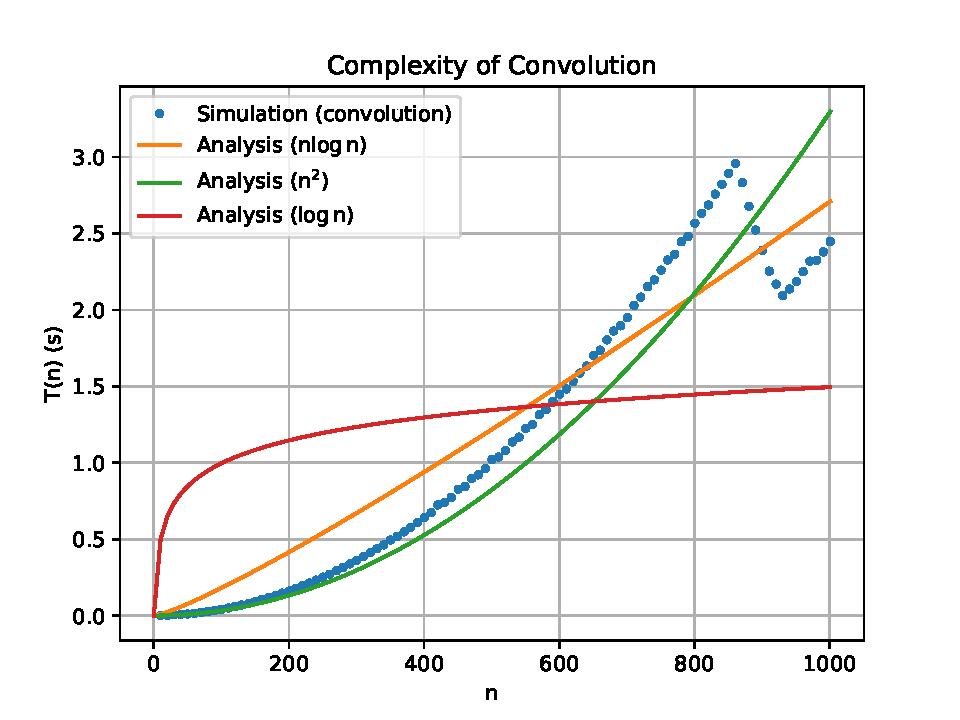
\includegraphics[width=\columnwidth]{Figure_15.pdf}
\end{center}
\captionof{figure}{}
\label{fig:15}	
\end{figure}

\begin{figure}[!ht]
\begin{center}
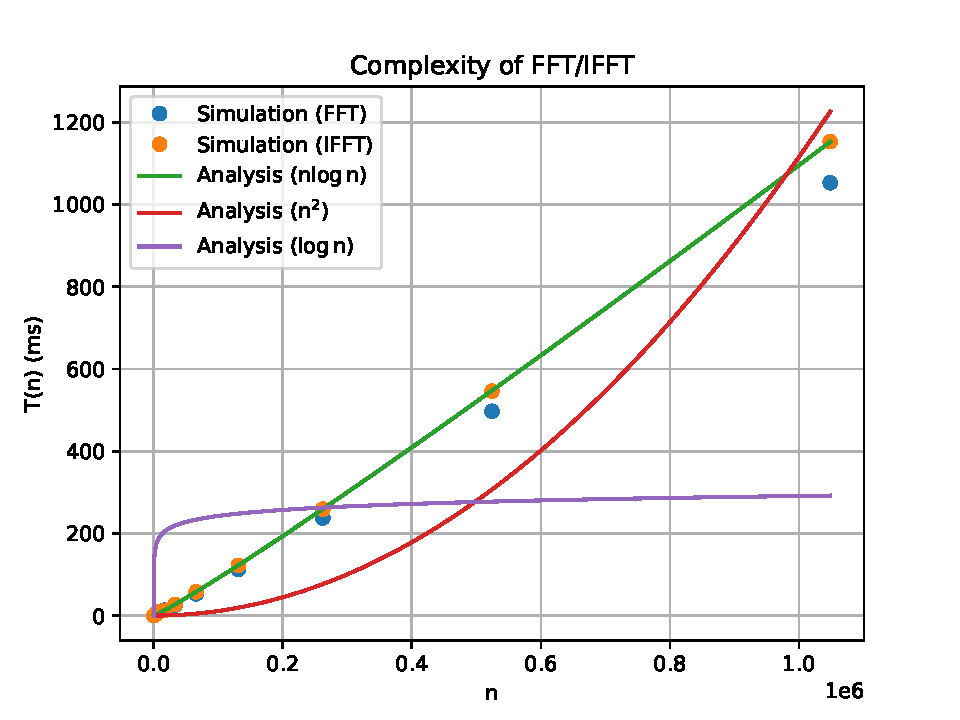
\includegraphics[width=\columnwidth]{Figure_16.pdf}
\end{center}
\captionof{figure}{}
\label{fig:16}	
\end{figure}
\end{enumerate}



\section{Exercises}
Answer the following questions by looking at the python code in Problem \ref{prob:output}.
\begin{enumerate}[label=\thesection.\arabic*]
\item
The command
\begin{lstlisting}
	output_signal = signal.lfilter(b, a, input_signal)
	\end{lstlisting}
in Problem \ref{prob:output} is executed through the following difference equation
\begin{equation}
\label{eq:iir_filter_gen}
 \sum _{m=0}^{M}a\brak{m}y\brak{n-m}=\sum _{k=0}^{N}b\brak{k}x\brak{n-k}
\end{equation}
%
where the input signal is $x(n)$ and the output signal is $y(n)$ with initial values all 0. Replace
\textbf{signal.filtfilt} with your own routine and verify.\\
\solution The following code executes the above question.
\begin{lstlisting}
wget https://github.com/anitadash/EE3900/blob/main/Codes/8_1.py
\end{lstlisting}

%
\item Repeat all the exercises in the previous sections for the above $a$ and $b$.\\
\solution
For the given values, the difference equation is
\begin{align}
	&y(n) - \brak{2.52}y(n - 1) + \brak{2.56}y(n - 2) \nonumber \\
	&- \brak{1.21}y(n - 3) + \brak{0.22}y(n - 4) \nonumber \\
	&= \brak{3.45 \times 10^{-3}}x(n) + \brak{1.38 \times 10^{-2}}x(n - 1) \nonumber \\
	&+ \brak{2.07 \times 10^{-2}}x(n - 2) + \brak{1.38 \times 10^{-2}}x(n - 3) \nonumber \\
	&+ \brak{3.45 \times 10^{-3}}x(n - 4)
\end{align}
From \eqref{eq:iir_filter_gen}, we see that the transfer function can be written as follows
\begin{align}
	H(z) &= \frac{\sum_{k = 0}^{N}b(k)z^{-k}}{\sum_{k = 0}^{M}a(k)z^{-k}} \\
		 &= \sum_{i}\frac{r(i)}{1 - p(i)z^{-1}} + \sum_{j}k(j)z^{-j}
	\label{eq:trans-func}
\end{align}
where $r(i)$, $p(i)$, are called residues and poles respectively of the partial 
fraction expansion of $H(z)$. $k(i)$ are the coefficients of the direct polynomial 
terms that might be left over. We can now take the inverse $z$-transform of
\eqref{eq:trans-func} and get using \eqref{eq:anun},
\begin{align}
	h(n) &= \sum_{i}r(i)[p(i)]^nu(n) + \sum_{j}k(j)\delta(n - j)
	\label{eq:h-n-expr}
\end{align}
Substituting the values,
\begin{align}
	&h(n) = [\brak{-0.24-0.71\j}\brak{0.56+0.14\j}^n \nonumber \\
	&+ \brak{-0.24+0.71\j}\brak{0.56-0.14\j}^n \nonumber \\
	&+ \brak{-0.25+0.12\j}\brak{0.70+0.41\j}^n \nonumber \\
	&+ \brak{-0.25-0.12\j}\brak{0.70-0.41\j}^n]u(n) \nonumber \\
	&+ \brak{1.6 \times 10^{-2}}\delta(n) \\
	&\implies h(n) = \brak{1.5}\brak{0.58}^n\cos\brak{n\alpha_1 + \beta_1} \nonumber \\
	&+ \brak{0.55}\brak{0.81}^n\cos\brak{n\alpha_2 + \beta_2} \nonumber \\
	&+ \brak{1.6 \times 10^{-2}}\delta(n)
	\label{eq:h-n-real}
\end{align}
where
\begin{align}
	\tan{\alpha_1} &= 0.25 \\
	\tan{\beta_1} &= 2.96 \\
	\tan{\alpha_2} &= 0.59 \\
	\tan{\beta_2} &= -0.48
	\label{eq:h-params}
\end{align}
The values $r(i)$, $p(i)$, $k(i)$ and thus below is the code for the impulse response function 
\begin{lstlisting}
wget https://github.com/anitadash/EE3900/blob/main/Codes/8_2_1.py
\end{lstlisting}
code for the filter frequency response.
\begin{lstlisting}
wget https://github.com/anitadash/EE3900/blob/main/Codes/8_2_2.py
\end{lstlisting}
Observe that for a series $t_n = r^n$, $\frac{t_{n + 1}}{t_n} = r$.
By the ratio test, $t_n$ converges if $|r| < 1$. We observe that for all $i$, 
$|p(i)| < 1$ and so, as $h(n)$ is the sum of many convergent series,
we see that $h(n)$ converges and is bounded. From \eqref{eq:z_trans},
\begin{align}
	\sum_{n = 0}^{\infty}h(n) = H(1) = \frac{\sum_{k = 0}^{N}b(k)}{\sum_{k = 0}^{M}a(k)} = 1 < \infty
\end{align}
Therefore, the system is stable. From
Fig. \eqref{fig:butter-imp}, $h(n)$ is negligible after $n \geq 64$, and we
can apply a 64-bit FFT to get y(n). The following code uses the DFT matrix
to generate $y(n)$ in Fig. \eqref{fig:19}
\begin{lstlisting}
wget https://github.com/anitadash/EE3900/blob/main/Codes/8_2_3.py
\end{lstlisting}
\begin{figure}[!ht]
\begin{center}
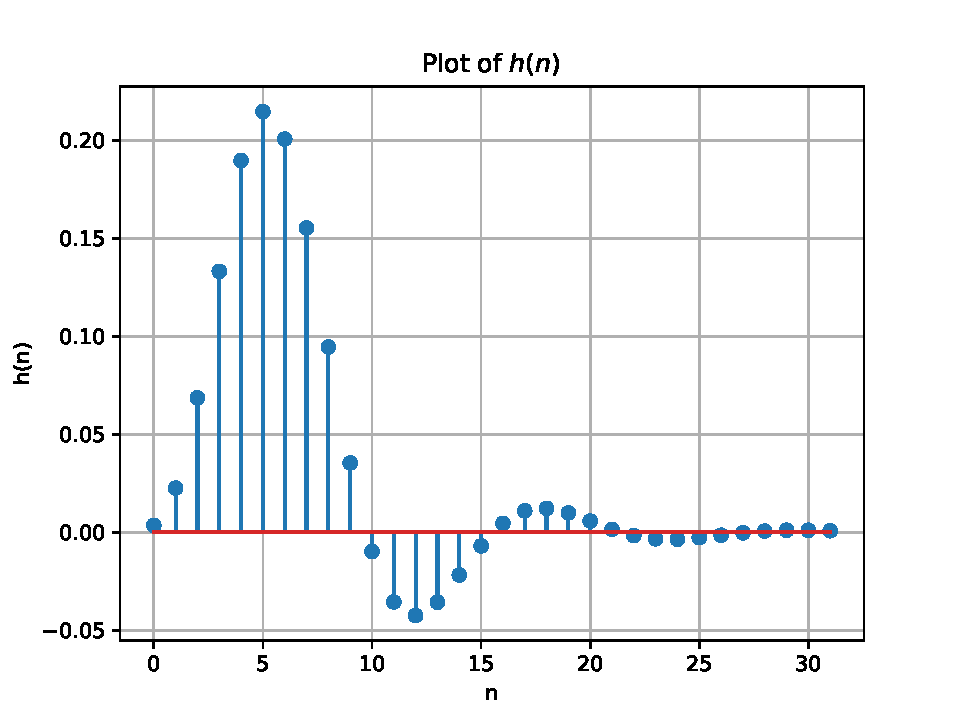
\includegraphics[width=\columnwidth]{Figure_17.pdf}
\end{center}
\captionof{figure}{}
\label{fig:17}	
\end{figure}
\begin{figure}[!ht]
\begin{center}
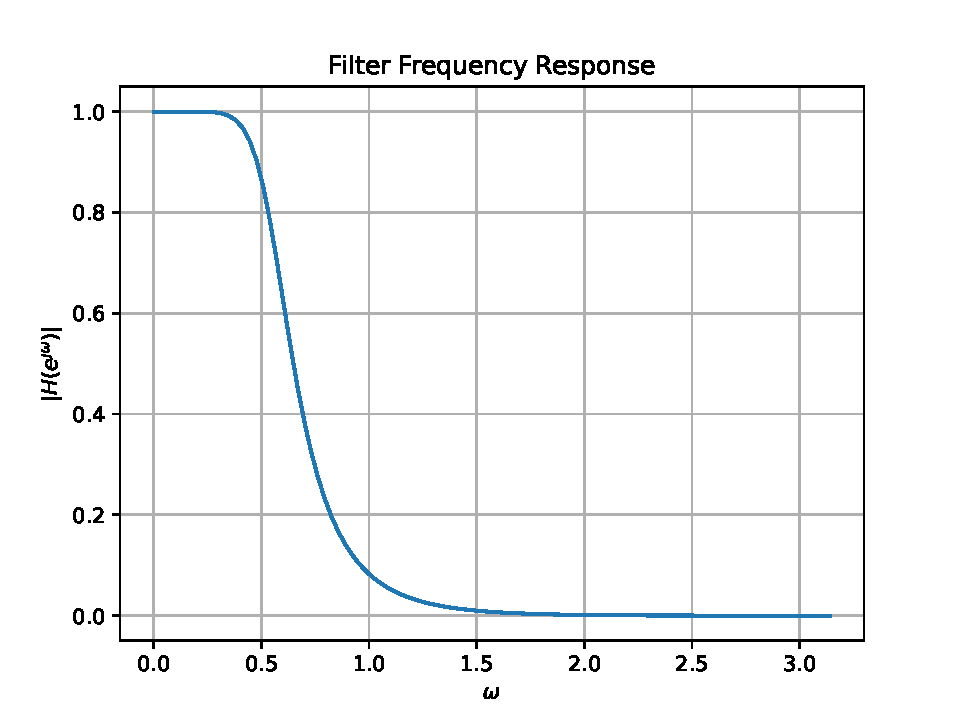
\includegraphics[width=\columnwidth]{Figure_18.pdf}
\end{center}
\captionof{figure}{}
\label{fig:18}	
\end{figure}
\begin{figure}[!ht]
\begin{center}
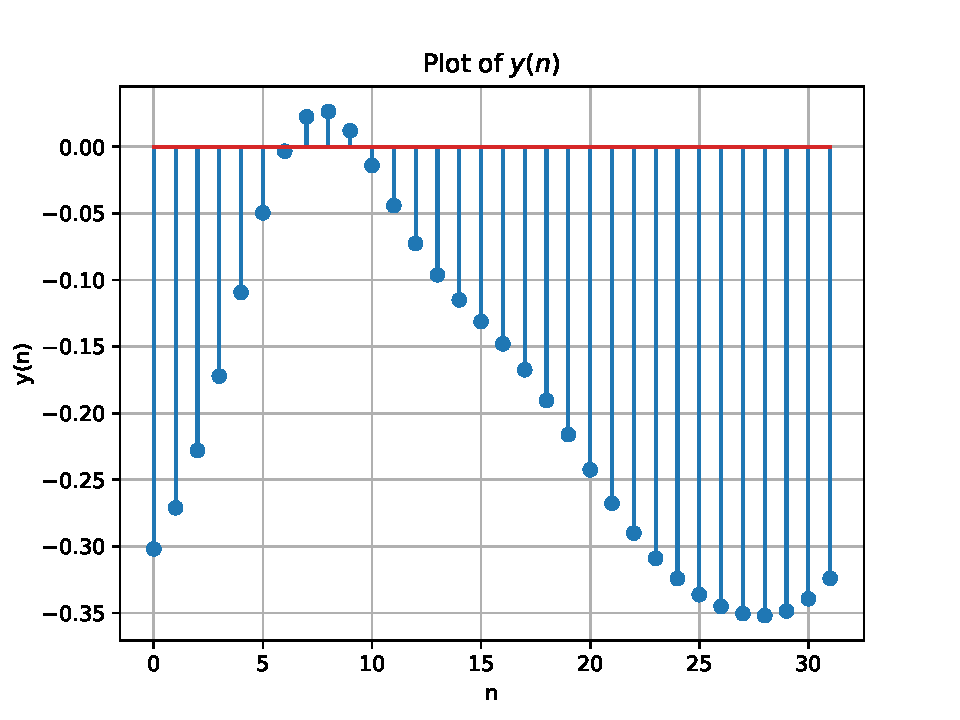
\includegraphics[width=\columnwidth]{Figure_19.pdf}
\end{center}
\captionof{figure}{}
\label{fig:19}	
\end{figure}
\item What is the sampling frequency of the input signal?
\\
\solution
Sampling frequency(fs)=44.1kHZ.
\item
What is type, order and  cutoff-frequency of the above butterworth filter
\\
\solution
The given butterworth filter is low pass with order=2 and cutoff-frequency=4kHz.
%
\item
Modifying the code with different input parameters and to get the best possible output.\\
\solution
A better filtering was found on setting the order of the filter to be 7.
\end{enumerate}

\end{document}


